\documentclass[a4paper,11pt,fleqn]{report}
% \usepackage[swedish]{babel}
\usepackage[T1]{fontenc}
\usepackage{latexsym}
\usepackage{amssymb} % F�r dubbelpilar etc
\usepackage{graphicx}
\usepackage{float}
\usepackage{psfrag}

\frenchspacing

\author{Daniel Uppstr�m}
\title{Wavelets Applied}
\date{2005-2006}
\begin{document}
\addtolength{\hoffset}{-20pt}
\addtolength{\textwidth}{+30pt}
\maketitle

\chapter*{Preface}
This paper is the result of a master thesis work in applied mathematics at G�teborg University. From the beginning, the purpose was to find a way to detect the presence of speech in an audio signal with the use of wavelets. During the investigation it turned out that this was a field where some features of the wavelet transform could be used, but the gain of expanding the audio directly into wavelets was not obvious. Focus was therefore shifted to other areas where wavelets could be useful, e.g. to the solution of differential equations. It was also investigated how wavelets could be used to invert the Radon transform, associated to medical imaging. This paper should therefore, in essence, be considered as a discussion about applications of wavelets.\\
I would like to thank my supervisor, professor J�ran Bergh, for his patience and interesting comments, that made this thesis work educational.\\
\\2006-05\\
\\Daniel Uppstr�m 
   
\tableofcontents

\chapter{Starting Point}

\section{Introduction}

In this first chapter some notational technicalities are mentioned. There are also some important definitions given that are used throughout this thesis. Chapter 2 features a brief and formal introduction to the theory of wavelets and multiresolution analysis. For a more pedagogical introduction to the subject see e.g. \cite{Strang}, \cite{Bergh} or \cite{Goswami}. A detailed textbook on the subject of functional analysis and Hilbert space theory can be found in \cite{Debnath}.

\section{Mathematical Notation and some Definitions}

Throughout this thesis, an integration without specified limits is assumed to be over the whole space in which the integrand is defined. I.e. for a function f defined in ${\mathbb R}$,
\begin{displaymath}
\displaystyle \int f(t)\ dt= \int_{-\infty}^{+\infty} f(t)\ dt.
\end{displaymath}
The Fourier transform of a function $f \in L^1({\mathbb R})$ is defined as
\begin{displaymath}
\widehat{f}(\omega)=\frac{1}{\sqrt{2\pi}}\int f(t)\ e^{-i\omega t}\ dt.
\end{displaymath}
This is extended to $L^2({\mathbb R})$ by introducing a sequence of continuous functions with compact support convergent to $f$ in $L^2({\mathbb R})$, i.e. ${\|f_n-f\|_2\rightarrow 0}$. The Fourier transform of $f\in L^2({\mathbb R})$ is then
\begin{displaymath}
\widehat{f}=\lim_{n\rightarrow \infty}\ \widehat{f}_n.
\end{displaymath}
The inverse transform is defined as
\begin{displaymath}
f(t)=\lim_{n\rightarrow \infty}\ \frac{1}{\sqrt{2\pi}}\ \int_{-n}^n \widehat{f}(\omega)\ e^{i\omega t}\ d\omega .
\end{displaymath} 
When working in discrete domain, the z-transform of a series $(a_k)$ is defined as
\begin{displaymath}
A(z)=\sum_k a_k\,z^{-k}.
\end{displaymath} 
Substituting $e^{i\omega}$ for $z$ gives the discrete Fourier transform
\begin{displaymath}
A(\omega)=\sum_k a_k\,e^{-i\omega k}.
\end{displaymath}
The inner-product of two functions $f$ and $g$ is written $\langle f,g \rangle$ and, if e.g. $f,g \in L^2({\mathbb R})$, then
\begin{displaymath}
\langle f,g \rangle = \displaystyle \int f(t)\,\overline{g(t)}\ dt.
\end{displaymath}
The norm of a function $f$ belonging to any inner-product space is defined by
\begin{displaymath}
\|f\|=\sqrt{\langle f,f \rangle}.
\end{displaymath}
The domain of a function $f$ or operator $A$ is denoted by $\mathcal{D}(f)$ or $\mathcal{D}(A)$ respectively. The range is written like $\mathcal{R}(f)$ and $\mathcal{R}(A)$. The null space is $\mathcal{N}(f)$, i.e. for an $x\in\mathcal{N}(f)$, $f(x)=0$, where $0$ is the zero element in the set $\mathcal{R}(f)$. The adjoint of an operator A is denoted $A^*$.

\section{Differential Equations}
Consider the ordinary formulation of an equation
\begin{displaymath}
Tu=f
\end{displaymath}
where $T$ is a differential operator, $f$ some given function and $u$ the unknown solution.
 To solve this equation it is common to look for an (approximate) solution $U$ in terms of basis vectors that spans some \emph{trial space} $V$. In the variational formulation, one search for a solution such that the error is orthogonal to a \emph{test space} $W$. I.e., the equivalent formulation is to find $U\in V$ such that
\begin{displaymath}
\langle TU-f,w \rangle=0
\end{displaymath}
or
\begin{equation}\label{varform}
\langle TU,w \rangle=\langle f,w \rangle
\end{equation}
for every $w\in W$.  \\
The trial and test spaces can be chosen according to boundary conditions and/or numerical aspects. In many cases they are the same, $V=W$.\\
When there are $M$ basis vectors spanning $V$ and $N$ vectors in the basis for $W$, equation (\ref{varform}) is equivalent to
\begin{displaymath}
\sum_{i=1}^{M}\sum_{j=1}^{N}\ \xi_i\,\langle Tv_i,w_j \rangle = \sum_{i=1}^{N}\ \langle f,w_k \rangle.
\end{displaymath}
In matrix form,
\begin{equation}\label{matrform}
A\,\xi=b
\end{equation}
where A is the matrix representation of the operator $T$ in the trial and test spaces and is known as the $M\times N$ \emph{stiffness matrix} given by
\begin{displaymath}
A_{i,j}= \langle Tv_i,w_j \rangle,
\end{displaymath}
$\xi$ is a vector of $M$ unknown coefficients for the solution in terms of $\{v_i\}_{i=1}^M$ and $b$ is the \emph{load vector} defined by
\begin{displaymath}
b_i= \langle f,w_i \rangle,\quad i=1,\ldots,M.
\end{displaymath}
If the basis vectors are highly localized elements with compact support, the matrix $A$ will only have a diagonal band of entries different from zero, which makes it easily inverted and (\ref{matrform}) can be solved readily. This is known as Galerkin's method.\\

\chapter{Fundamental Wavelet Theory}
\section{Scaling Functions and Spaces}
Let $V_j$ be a set of closed subspaces of $L^2({\mathbb R})$ with the following properties:
\begin{enumerate}
\item
$V_j \subset V_{j+1}\ \forall\ j\in{\mathbb Z}$,
\item
$f(t) \in V_j \Leftrightarrow f(2t)\in V_{j+1}\ \forall\ j\in{\mathbb Z}$,
\item
$\overline{\cup_j V_j}=L^2({\mathbb R})$,
\item
$\cap_j V_j = \{0\}$,
\item
$\exists$ a \emph{scaling function} $\phi\in V_0$, such that $\{\phi(t-k)\}_{k\in{\mathbb Z}}$ is a Riesz basis for $V_0$.
\end{enumerate} 
Now, for a given $\phi(t)$, denote its dilated, translated and normalized replicas as
\begin{displaymath}
\phi_{j,k}(t)=2^{j/2}\phi(2^jt-k).
\end{displaymath}
Then $\|\phi_{j,k}\|=\|\phi\|$ and, for each $j$, $\{\phi_{j,k}\}_{k\in{\mathbb Z}}$ is a basis for $V_j$.\\
The first condition now implies that
\begin{equation} \label{scaleq}
\underbrace{\phi(t)}_{\in V_0}=2\sum_k\ h_k\ \underbrace{\phi(2t-k)}_{\in V_1}
\end{equation}
for some coefficients $(h_k)$. This is known as the scaling equation.\\
In Fourier domain it corresponds to
\begin{equation} \label{scaleqf}
\widehat{\phi}(\omega) = H(\omega/2)\ \widehat{\phi}(\omega/2),
\end{equation}
where
\begin{displaymath}
H(\omega)= \sum_k\ h_k\ e^{-ik\omega}.
\end{displaymath}
Let also the scaling function have integral equal to unity,
\begin{displaymath}
\int\phi(t)\ dt = 1
\end{displaymath}
or equivalently,
\begin{displaymath}
\widehat{\phi}(0)=1.
\end{displaymath}
Equation (\ref{scaleqf}) then implies
\begin{equation} \label{hsum}
\sum_k\ h_k =1.
\end{equation}
The most trivial function satisfying these criteria is the Haar scaling function given by:
\begin{displaymath}
\phi(t)= \left \{ \begin{array}{ll} 1 & \textrm{if $0<t<1$,}\\
                              0 & \textrm{otherwise.}
\end{array} \right.
\end{displaymath}
The corresponding coefficients are then $h_0=\frac{1}{2}$ and $h_1=\frac{1}{2}$.

\section{Wavelets and Detail Spaces} 
Denote the projections of an arbitrary function $f$ onto the spaces $V_j$ and $V_{j+1}$ by $f_j$ and $f_{j+1}$ respectively. Since $V_j\subset V_{j+1}$, $f_{j+1}$ is a more detailed approximation (of $f$) than $f_j$. Denote the difference $d_j$, i.e.
\begin{displaymath}
d_j=f_{j+1}-f_j.
\end{displaymath}
Now introduce the space $W_j$ such that $d_j \in W_j$. This means that $W_j\subset V_{j+1}$ and $V_j\oplus W_j=V_{j+1}$. The space $W_j$ is then known as a detail space of level j. \\
Next, introduce a \emph{wavelet} $\psi(t)$ such that $\{\psi(t-k)\}_{k\in{\mathbb Z}}$ is a basis of $W_0$. Then
\begin{equation} \label{waveeq}
\psi(t)=2\sum_k\ g_k\ \phi(2t-k)
\end{equation}
for some coefficients $(g_k)$. This is known as the wavelet equation.\\
In Fourier domain it corresponds to
\begin{equation} \label{waveeqf}
\widehat{\psi}(\omega) = G(\omega/2)\ \widehat{\phi}(\omega/2),
\end{equation}
where
\begin{displaymath}
G(\omega)= \sum_k\ g_k\ e^{-ik\omega}.
\end{displaymath}
Furthermore, the wavelet has vanishing integral,
\begin{displaymath}
\int\psi(t)\ dt = 0
\end{displaymath}
or equivalently,
\begin{displaymath}
\widehat{\psi}(0)=0.
\end{displaymath}
Equation (\ref{waveeqf}) and $\widehat{\phi}(0)=1$ then implies
\begin{equation} \label{gsum}
\sum_k\ g_k =0.
\end{equation}
The simplest function satisfying these criteria is the Haar wavelet given by:
\begin{displaymath}
\psi(t)= \left \{ \begin{array}{ll} 1 & \textrm{if $0<t<\frac{1}{2}$,}\\
                              -1 & \textrm{if $\frac{1}{2}<t<1$,}\\
			      0 & \textrm{otherwise.}
\end{array} \right.
\end{displaymath}
The corresponding coefficients are $g_0=\frac{1}{2}$ and $g_1=-\frac{1}{2}$.

\section{Wavelet Decomposition}
From the definitions above it follows that any $f\in L^2({\mathbb R})$ can be described by its projection on some coarse level $j_0$ of scaling space, $V_{j_0}$, together with its projections on detail spaces $W_{j_0}$, $W_{j_0+1}$, $W_{j_0+2}$ and so on. I.e.,
\begin{displaymath}
f \approx \sum_k s_{j_0,k}\ \phi_{j_0,k} + \sum_k \omega_{j_0+1,k}\ \psi_{j_0+1,k} + \sum_k \omega_{j_0+2,k}\ \psi_{j_0+2,k} + \ldots
\end{displaymath}
or, more formal,
\begin{equation}\label{decomp}
f \approx \sum_k s_{j_0,k}\ \phi_{j_0,k} + \sum_{j=j_0}^J \sum_k \omega_{j,k}\ \psi_{j,k},
\end{equation}
where $J$ is some fine level of resolution.
The spaces $(V_j)$ and $(W_j)$ are then said to constitute a \emph{Multiresolution Analysis} (MRA) and (\ref{decomp}) is the corresponding Wavelet decomposition.


\section{Orthogonality}
From the previous sections $V_j \subset V_{j+1}$, $W_j \subset V_{j+1}$ and $W_j\ \bot\ V_j$ . Thus 
\begin{displaymath}
\langle\psi_{J,k},\phi_{j,l}\rangle=0\quad \forall\ j\le J
\end{displaymath}
and
\begin{displaymath}
\langle\psi_{J,k},\psi_{j,l}\rangle=0\quad \forall\ j\ne J.
\end{displaymath}
But so far, nothing is said about orthogonality between scaling or detail functions in the same level. In the general case it is always possible to introduce the dual MRA with spaces $\widetilde{V}_j$ and $\widetilde{W}_j$ spanned by $\widetilde{\phi}_{j,k}$ and $\widetilde{\psi}_{j,k}$ such that
\begin{displaymath}
\langle\phi_{j,k},\widetilde{\phi}_{j,l}\rangle=\delta_{k,l}\\
\end{displaymath}
\begin{displaymath}
\langle\psi_{j,k},\widetilde{\psi}_{j,l}\rangle=\delta_{k,l}\\
\end{displaymath}
\begin{displaymath}
\langle\phi_{j,k},\widetilde{\psi}_{j,l}\rangle=0.
\end{displaymath}
In some cases the MRA is self-dual and
\begin{displaymath}
\widetilde{\phi}=\phi
\end{displaymath}
\begin{displaymath}
\widetilde{\psi}=\psi.
\end{displaymath}
This is then referred to as an orthogonal MRA. In the more general case, the two MRA's are said to be biorthogonal.\\
Note that the dual functions have their equivalents to (\ref{scaleq}) and (\ref{waveeq}):
\begin{equation} \label{dscaleq}
\widetilde{\phi}(t)=2\sum_k\ \widetilde{h}_k\ \widetilde{\phi}(2t-k)
\end{equation}
\begin{equation} \label{dwaveeq}
\widetilde{\psi}(t)=2\sum_k\ \widetilde{g}_k\ \widetilde{\phi}(2t-k)
\end{equation}

\section{The Forward Wavelet Transform}
Assume that a function $f$ is known in terms of scaling coefficients at some fine scale $J$:
\begin{displaymath}
f = \sum_k s_{J,k}\ \phi_{J,k}
\end{displaymath}
But, $V_{J}=V_{J-1}\oplus W_{J-1}$, and f can be further expanded in terms of scaling and wavelet coefficients at level $J-1$:
\begin{equation}\label{spliteq}
\sum_k s_{J,k}\ \phi_{J,k}=\sum_k s_{J-1,k}\ \phi_{J-1,k}+\sum_k \omega_{J-1,k}\ \psi_{J-1,k}
\end{equation}
Taking the inner product with $\widetilde{\phi}_{J-1,l}$ and $\widetilde{\psi}_{J-1,l}$ respectively gives
\begin{displaymath}
s_{J-1,l}=\sum_k s_{J,k}\ \langle\phi_{J,k},\widetilde{\phi}_{J-1,l}\rangle
\end{displaymath}
and
\begin{displaymath}
\omega_{J-1,l}=\sum_k s_{J,k}\ \langle\phi_{J,k},\widetilde{\psi}_{J-1,l}\rangle.
\end{displaymath}
The inner products could be evaluated by the use of (\ref{dscaleq}) and (\ref{dwaveeq}) to get
\begin{displaymath}
\langle\phi_{J,k},\widetilde{\phi}_{J-1,l}\rangle = \sqrt{2}\ \sum_m \widetilde{h}_m\ \langle\phi_{J,k},\widetilde{\phi}_{J,m+2l}\rangle=\sqrt{2}\  \widetilde{h}_{k-2l}
\end{displaymath}
\begin{displaymath}
\langle\phi_{J,k},\widetilde{\psi}_{J-1,l}\rangle = \sqrt{2}\ \sum_m \widetilde{g}_m\ \langle\phi_{J,k},\widetilde{\phi}_{J,m+2l}\rangle=\sqrt{2}\  \widetilde{g}_{k-2l}.
\end{displaymath}
And thus,
\begin{equation}\label{fwts}
s_{J-1,l}=\sqrt{2}\ \sum_k s_{J,k}\ \widetilde{h}_{k-2l}
\end{equation}
\begin{equation}\label{fwtw}
\omega_{J-1,l}=\sqrt{2}\ \sum_k s_{J,k}\ \widetilde{g}_{k-2l}.
\end{equation}
Keeping the wavelet coefficients while repeating the procedure with the new scaling coefficients recursively, gives a sequence of wavelet coefficients at decreasing resolutions together with scaling coefficients at some coarse level where the iterations are stopped. This gives (\ref{decomp}) and is known as the (Fast) Forward Wavelet Transform (FWT).\\
The inverse transform is similarly implemented. Using (\ref{scaleq}) and (\ref{waveeq}), (\ref{spliteq}) can be written as
\begin{displaymath}
\sum_k s_{J,k}\, \phi_{J,k}=\sqrt{2}\ \sum_k s_{J-1,k}\ \sum_l h_l\, \phi_{J,l+2k}+\sqrt{2}\ \sum_k \omega_{J-1,k}\ \sum_l g_l\, \phi_{J,l+2k}.
\end{displaymath}
Taking inner product with $\widetilde{\phi}_{J,k}$ and rearranging while keeping track of the indices gives
\begin{equation}\label{ifwt}
s_{J,k}=\sqrt{2}\ \sum_l s_{J-1,l}\ h_{k-2l} + \sqrt{2}\ \sum_l \omega_{J-1,l}\ g_{k-2l}.
\end{equation}
Repeating this recursively gives scaling coefficients of increasing resolution.


\section{Filter Banks and Subsampling}
The recursive operations in the FWT can be seen as convolutions between scaling coefficients and the reversed sequences of $(\sqrt{2}\ \widetilde{h}_k)$ and $(\sqrt{2}\ \widetilde{g}_k)$. But in signal processing, a convolution with a sequence, say $(a_k)$, is equivalent to applying a filter with impulse response $(a_{-k})$. If the downsampling operator $(\downarrow2)$ is defined to remove all elements with odd indices in a series, i.e. $(a_k)\rightarrow(a_{2k})$, equations (\ref{fwts}) and (\ref{fwtw}) can be visualized by a simple filter bank.   


\begin{figure}[H]
\centering
\psfrag{H*}[][]{$\widetilde{H}^*$}
\psfrag{G*}[][]{$\widetilde{G}^*$}
\psfrag{sJ}[][]{$s_J$}
\psfrag{sJ-1}{$s_{J-1}$}
\psfrag{wJ-1}{$\omega_{J-1}$}
\includegraphics[scale=0.6]{singlestep.eps}
\caption{Single-Step Analysis Filter Bank}
\label{ssanalysisbankfig}
\end{figure}
Here $\widetilde{H}^*$ and $\widetilde{G}^*$ are filters with impulse responses $(\sqrt{2}\ \widetilde{h}_{-k})$ and $(\sqrt{2}\ \widetilde{g}_{-k})$ respectively. Together with the downsampling operators they form a single-step analysis filter bank. By combining many of these units into a larger network one gets the FWT to a given level of resolution ($J-3$ in the figure).
\begin{figure}[H]
\centering
\psfrag{H*}[][]{$\widetilde{H}^*$}
\psfrag{G*}[][]{$\widetilde{G}^*$}
\psfrag{sJ}[][]{$s_J$}
\psfrag{sJ-1}{$s_{J-1}$}
\psfrag{wJ-1}{$\omega_{J-1}$}
\psfrag{wJ-2}{$\omega_{J-2}$}
\psfrag{wJ-3}{$\omega_{J-3}$}
\psfrag{sJ-3}{$s_{J-3}$}
\includegraphics[scale=0.5]{fwt.eps}
\caption{The Forward Wavelet Transform}
\label{FWTbankfig}
\end{figure}
Now, define the upsampling operator $(\uparrow 2)$ to insert a zero between every element in a series, i.e. $(a_k)\rightarrow(\ldots,a_{-2},0,a_{-1},0,a_0,0,a_1,0,a_2,\ldots)$. The inverse transform defined by subsequent application of (\ref{ifwt}), can then be visualized in a similar way.
\begin{figure}[H]
\centering
\psfrag{H}[][]{$H$}
\psfrag{G}[][]{$G$}
\psfrag{sJ}[][]{$s_J$}
\psfrag{sJ-1}[][]{$s_{J-1}$}
\psfrag{wJ-1}[][]{$\omega_{J-1}$}
\psfrag{wJ-2}[][]{$\omega_{J-2}$}
\psfrag{wJ-3}[][]{$\omega_{J-3}$}
\psfrag{sJ-3}[][]{$s_{J-3}$}
\includegraphics[scale=0.5]{ifwt.eps}
\caption{The Inverse Wavelet Transform}
\label{IFWTbankfig}
\end{figure}
Here $H$ and $G$ are filters with impulse responses $(\sqrt{2}\ h_{k})$ and $(\sqrt{2}\ g_{k})$. These are known as the synthesis filters. Note that in the orthogonal case $\widetilde{H}=H$ and $\widetilde{G}=G$ and thus the impulse responses of the analysis filters are time reverses of the impulse responses of the synthesis filters.\\
If a unit of the analysis bank is connected directly to a synthesis bank unit, the resulting network should be equivalent to the identity operator.
\begin{figure}[H]
\centering
\psfrag{H*}[][]{$\widetilde{H}^*$}
\psfrag{G*}[][]{$\widetilde{G}^*$}
\psfrag{H}[][]{$H$}
\psfrag{G}[][]{$G$}
\psfrag{x}[][]{$x$}
\psfrag{xhat}{$\widehat{x}$}
\includegraphics[scale=0.5]{reconstruction.eps}
\caption{Analysis + Synthesis}
\label{reconstructionfig}
\end{figure}
The requirements that this places on the filters are directly translated to the coefficient in the scaling and wavelet equations. This can be used in the construction of wavelets and scaling functions. \\
Switching to z-domain turns the convolution done in a filter into multiplication. The effect of the subsampling operators (i.e. down- and upsampling) in z-domain can be calculated with some minor effort. Let $y=(\downarrow 2)\,x$. Then 
\begin{displaymath}
Y(z)=\frac{1}{2}\,[X(z^{1/2})+X(-z^{1/2})]
\end{displaymath}
and, for $u=(\uparrow 2)\,x$,
\begin{displaymath}
U(z)=X(z^2).
\end{displaymath}
Applying both operators in sequence like $v=(\uparrow 2)(\downarrow 2)\,x$ gives
\begin{displaymath}
V(z)=\frac{1}{2}\,[X(z)+X(-z)].
\end{displaymath}
Now, for the input and output sequences in figure \ref{reconstructionfig} one gets 
\begin{displaymath}
\widehat{X}(z)=\frac{1}{2}\,[H(z)\widetilde{H}^*(z)+G(z)\widetilde{G}^*(z)]X(z)+\frac{1}{2}\,[H(z)\widetilde{H}^*(-z)+G(z)\widetilde{G}^*(-z)]X(-z).
\end{displaymath}
To get perfect reconstruction, i.e. $\widehat{X}(z)=X(z)$, the filters must satisfy the following two conditions
\begin{displaymath}
H(z)\widetilde{H}^*(z)+G(z)\widetilde{G}^*(z)=2,
\end{displaymath}
\begin{displaymath}
H(z)\widetilde{H}^*(-z)+G(z)\widetilde{G}^*(-z)=0.
\end{displaymath}
The first means no distortion and the second ensures alias cancellation. Filters satisfying these criteria are known as \emph{quadrature mirror filters} of which there are many presented in the literature, giving rise to different families of wavelets and scaling functions \cite{Strang}.


\section{Higher dimensions}
A lot of successful applications involving wavelets are related to image processing. Since an image is (most often) two dimensional, some modifications of the previously described multiresolution analysis are needed. The most popular approach is probably to use simple tensor products of one-dimensional wavelets and scaling functions.
\begin{displaymath}
\Phi(x,y)=\phi(x)\phi(y)
\end{displaymath}
\begin{displaymath}
\Psi^{(1)}(x,y)=\phi(x)\psi(y)
\end{displaymath}
\begin{displaymath}
\Psi^{(2)}(x,y)=\psi(x)\phi(y)
\end{displaymath}
\begin{displaymath}
\Psi^{(3)}(x,y)=\psi(x)\psi(y)
\end{displaymath}
The three wavelets capture details in the two Cartesian coordinates and at the diagonal, respectively.
The main drawback with this simple approach is that there is little invariance with respect to rotation. If this is a problem one can use non-separable wavelets with other properties. See e.g. \cite{Bergh}.  


\chapter{Operators on an MRA}

The problem of finding the inverse of an operator covers differential equations as well as transform inversion and many other problems in applied mathematics. Wavelets have prove to be useful as a basis for diagonalization of many operators and have some interesting advantages compared to the very unlocalized terms of a Fourier series and, at the other end, localized finite element bases. This is exemplified in \cite{Soveiko} where scaling functions and wavelets (from a single fixed scale though) are used in harmonic balance calculations of high-frequency electronic circuits. An area that has almost exclusively relied on the Fourier transform but where computations get costly with many excitation tones or complex waveforms. This is where wavelets seem to come in handy. The paper by Xin Li et al. \cite{Li} also highlights these advantages. 
   
\section{Wavelet Diagonalization}
One major advantage of wavelets from an MRA over simple finite-element functions is due to their orthogonality between different scales. To finite elements there is always an associated mesh which needs to be properly defined, and often subsequently refined, in order to get sufficient details visible in the solution at a low computational cost. Wavelets on the other hand, provide a multiresolution basis by their translation and dilation properties. By orthogonality, different levels in the MRA captures different levels of details in the solution simultaneously. Thus, for each scale, there is a built-in mesh, providing both advantages and disadvantages. \\
When the union of spaces $(V)$ and $(W)$ from some MRA are chosen both as trial and test space in the variational formulation of some equation, it is known as the Wavelet-Galerkin method.
\section{Discretization}
Consider the following equation,
\begin{equation}\label{nonlinode}
Lu=f
\end{equation}
where $L$ is a linear operator, $f$ some given function and $u$ the unknown solution. As stated in the previous section, in the Wavelet-Galerkin method one tries to represent the operator $L$ in terms of the bases from an (orthogonal) MRA. Then the nested structure is inherited to the operator representation and the operator can be represented by the coefficients
\begin{eqnarray}
\alpha_{j,k,l}=\langle L\psi_{j,k},\psi_{j,l} \rangle \nonumber \\
\beta_{j,k,l}=\langle L\phi_{j,k},\psi_{j,l} \rangle \nonumber \\
\gamma_{j,k,l}=\langle L\psi_{j,k},\phi_{j,l} \rangle \nonumber\\
s_{j,k,l}=\langle L\phi_{j,k},\phi_{j,l} \rangle.
\end{eqnarray}
Representing an operator by these nested series of coefficients is known as the non-standard form, to be compared with the standard matrix representation associated to the variational equation formulation.\\
By (\ref{fwts}) and (\ref{fwtw}) one gets
\begin{eqnarray}
\alpha_{j,k,l}=\sum_{m,n}\,g_m g_n s_{j-1,m-2k,n-2l} \nonumber \\
\beta_{j,k,l}=\sum_{m,n}\,h_m g_n s_{j-1,m-2k,n-2l} \nonumber \\
\gamma_{j,k,l}=\sum_{m,n}\,g_m h_n s_{j-1,m-2k,n-2l} \nonumber\\
s_{j,k,l}=\sum_{m,n}\,h_m h_n s_{j-1,m-2k,n-2l} 
\end{eqnarray}
Thus, once $\{s_{j,k,l}\}$ is known, the other coefficients are readily calculated.




\section{Quadrature}

Almost all wavelet applications depend on the expansion of some given function into scaling coefficients. This can be done in a number of ways, to give an error of known size. Consider the scaling coefficients of an orthogonal MRA,
\begin{eqnarray}\label{scaleonepoint}
s_{j,k}=\langle f,\phi_{j,k} \rangle= 2^{j/2} \int f(x)\,\phi(2^jx-k)\,dx=\nonumber\\
 = 2^{-j/2}\,\int f(2^{-j}(x+k))\,\phi(x)\,dx.
\end{eqnarray}
Thus, it is only necessary to find a quadrature formula for $\langle f,\phi_{0,0}\rangle$ and modify the argument of $f$ in the evaluation. 
In \cite{Beylkin1} Beylkin shows how the expansion of an arbitrary function into wavelets can be done if the scaling function is chosen such that it has a number of vanishing, shifted moments.
Let $\phi(x)$ be a scaling function that, for some integer constant $\tau_M$, satisfies
\begin{eqnarray}
\int \phi(x+\tau_M)\,x^m\,dx=0,\qquad m=1,2,\ldots,M-1,\label{shiftmom}\\
\int \phi(x)\,dx=1.\label{zeromomunity}
\end{eqnarray}
I.e. the first shifted moments of $\phi$ vanish, while the ``zeroth'' moment is equal to unity. Note that this is a property only satisfied by some (modified) scaling functions. The scaling coefficients associated with a given function $f$ can then be calculated by a simple Taylor series expansion. First consider the following modification of (\ref{scaleonepoint})
\begin{eqnarray}
s_{j,k}=\int f(x)\,\phi_{j,k}(x)\, dx\ =\ 2^{j/2} \int f(x)\,\phi(2^jx-k)\, dx\ =\nonumber\\
 =\ 2^{j/2} \int f(x+2^{-j}k)\,\phi(2^jx)\, dx =\nonumber\\=\ 2^{-j/2} \int f(2^{-j}(x+k))\,\phi(x)\, dx. \nonumber\\
\end{eqnarray}
Now expand $f$ into a Taylor series around $2^{-j}(k+\tau_M)$ and use (\ref{shiftmom}), (\ref{zeromomunity}) to get
\begin{equation}\label{s_Beylkin1}
s_{j,k}=2^{j/2}\, f(2^{-j}(k+\tau_M))+\mathcal{O}(2^{-j(M-\frac{1}{2})}).
\end{equation} 
A very neat one-point quadrature formula. Further expansion could then be done according to the FWT algorithm; (\ref{fwts}) and (\ref{fwtw}).\\
The same idea could be used to calculate stiffness matrix entries for integral operators. See \cite{Beylkin1} for further details.
For other bases without the property (\ref{shiftmom}) one needs another method. For instance, the expansion into scaling functions can be done with the use of Lagrange interpolating polynomials \cite{Johnson}. For the exact diagonalization of some common operators into arbitrary wavelets, see \cite{Beylkin2}.   
  
\section{Operator Biorthogonal Systems}\label{OBS}
An interesting feature associated to wavelets is that the standard MRA can be modified to suit the needs of a particular application. Especially it can be modified to diagonalize some (linear) operators. \\
For a given linear operator $A$ and orthogonal MRA $(\phi_{j,k})$ and $(\psi_{j,k})$, let $(u_{j,k})$, $(v_{j,k})$ and $(\tilde{u}_{j,k})$, $(\tilde{v}_{j,k})$ be a collection of functions such that 
\begin{eqnarray}
u_{j,k}=A\psi_{j,k}\nonumber\\ 
v_{j,k}=A\phi_{j,k}\nonumber
\end{eqnarray}
\begin{eqnarray}
A^*\tilde{u}_{j,k}=\psi_{j,k}\nonumber\\
A^*\tilde{v}_{j,k}=\phi_{j,k}\nonumber
\end{eqnarray}
Then
\begin{displaymath}
\langle u_{j,k},\tilde{u}_{j,l}\rangle= \langle A\psi_{j,k},\tilde{u}_{j,l}\rangle= \langle \psi_{j,k}, A^*\tilde{u}_{j,l}\rangle = \langle \psi_{j,k} ,\psi_{j,l}\rangle= \delta_{k,l}
\end{displaymath}
and, by the same argument,
\begin{displaymath}
\langle v_{j,k},\tilde{v}_{j,l}\rangle= \delta_{k,l}.
\end{displaymath}  
For shift-invariant operators, the functions $u$ and $v$ satisfy the scaling equations like
\begin{displaymath} 
u(t)= A\psi(t) = A(2\sum_k\ g_k\ \phi(2t-k))= 2\sum_k\ A(g_k\ \phi(2t-k))
\end{displaymath}
\begin{displaymath}
 = 2\sum_k\ g_k\ A\phi(2t-k)) = 2\sum_k\ g_k\ v(2t-k)
\end{displaymath}
and
\begin{displaymath} 
v(t)=\ ...\ = 2\sum_k\ h_k\ v(2t-k).
\end{displaymath}
Thus, one has a system of biorthogonal wavelet-like functions in which a given function can be expanded. This could be carried out by taking inner products with $\tilde{v}_{J,k}$ to get coefficients for $v_{J,k}$ and then following the standard FWT algorithm to get an expansion like
\begin{equation}
f=\sum_{j_0\le j<J,k}\langle f,\tilde{u}_{j,k} \rangle u_{j,k} + \sum_k \langle f,\tilde{v}_{j_0,k} \rangle v_{j_0,k}
\end{equation}
for some coarse level $j_0$.
In \cite{Donoho} Donoho calls these functions \emph{Vaguelettes} and the associated MRA a Wavelet-Vaguelette Decomposition (WVD).\\
Another operator biorthogonal system is introduced in \cite{Jawerth}. There a self-adjoint operator $L$ is decomposed into its square roots $L=VV$ which are used to form new wavelet-like bases $\Psi_{j,k}=V^{-1}\psi_{j,k}$ and $\widetilde{\Psi}_{j,k}=V^{-1}\widetilde{\psi}_{j,k}$, where $\psi_{j,k}$ and $\widetilde{\psi}_{j,k}$ are members of a biorthogonal MRA. The entries of the stiffness matrix then become
\begin{displaymath}
\langle L\Psi_{j,k},\widetilde{\Psi}_{j',l}\rangle = \langle V\Psi_{j,k},V\widetilde{\Psi}_{j',l}\rangle=\langle \psi_{j,k},\widetilde{\psi}_{j',l}\rangle=\delta_{j,j'}\delta_{k,l}.
\end{displaymath}
The case when $L=D^2$, the Laplace operator, is investigated in the article. Then $V^{-1}$ is the anti-derivative operator. Since the scaling function of a wavelet MRA never has vanishing (unshifted) moments, the corresponding $\Phi{j,k}=V^{-1}\phi_{j,k}$ does not have compact support in this case, which complicates matters. Nevertheless, the idea is interesting.


\chapter{One-Dimensional Signal Processing Applications}

\section{Stationary Oscillations}

If one wants to use the wavelet transform in applications like audio signal processing it is important to know how stationary oscillations, i.e. trigonometric functions, are described in wavelet domain. This will now be explained. \\ 
In an MRA connected to some discrete wavelet transform, the basis functions consists of wavelets and scaling functions that are both localized and most often compactly supported. In addition, the detail scales are fixed by dilation of integer powers of two. These restrictions might suggest that wavelets are not suitable to describe stationary oscillations. But from the definition of an MRA, the limit of the union of detail spaces is dense in $L^2$. This means that any function with finite energy can be described as a sum of wavelets. In reality it turns out that any stationary oscillation of a single fixed frequency and arbitrary phase could be roughly approximated by a sequence of wavelets in two (or better three) nearby scales.\\
Consider the following series
 \begin{displaymath}
\displaystyle f_1(t)=\sum_k \psi_{j,k}, 
\end{displaymath}
where $ \psi_{j,k}=\psi(2^jt-k) $, for some mother wavelet $\psi$ and scale $j$. With $\psi$ equal to the Haar wavelet $f(t)$ is a square wave with period $2^{-j}$ and angular frequency $\omega_1=2 \pi\ 2^j$. If $\psi$ is instead a reasonably smooth and symmetrical wavelet, the series could be approximated roughly as
 \begin{displaymath}
f_1(t)=\sin(\omega_1t+\phi).
\end{displaymath}
where $\phi$ is a phase term associated to the wavelet.\\
Now consider the series
\begin{displaymath}
\displaystyle f_2(t)=\sum_k(-1)^k\psi_{j,k}. 
\end{displaymath}
In the Haar case it corresponds to a square wave of period $2^{1-j}$ and frequency $\omega_2=2 \pi\ 2^{j-1}$ i.e. half the frequency of the first case. The phase is such that $t=0$ corresponds to the middle of a square and in the smoother case it could be written as
\begin{displaymath}
f_2(t)=\cos(\omega_2t+\phi_0)
\end{displaymath}
for some small $\phi_0$.
These arguments are justified by the following identity
\begin{equation}
\displaystyle \sum_k (-1)^k\psi(t-k)=\sum_l\psi(t/2-l+1/4).
\end{equation}
In an MRA, the coefficients of a stationary oscillation at the frequency $\omega=2 \pi\ 2^j$ and of arbitrary phase would be seen to contribute mostly in the two scales $j$ and $j+1$. In the coarser scale $j$ the coefficients will be of equal value $=a$ and sign whereas they will show up with equal value $=b$ but alternating sign in the more detailed scale $j+1$. The relationship between the numbers $a$ and $b$ is a measure of the phase of the wave such that
\begin{displaymath}
a\sin(\omega t+\phi)+b\cos(\omega t+\phi)=r\sin(\omega t+\phi+\theta)
\end{displaymath}  
where $r=\sqrt{a^2+b^2}$ and $\theta=\arctan(\frac{b}{a})$ if $a>0$ or $\theta=\pi+\arctan(\frac{b}{a})$ if $a<0$.\\
Now, consider the case where the frequency is different than a dyadic product of $2\pi$. This will obviously result in a more complex pattern in the MRA. If the frequency $\omega$ is such that $\frac{3}{4}\ 2\pi\ 2^j\lesssim\omega\lesssim\frac{6}{4}\ 2\pi\ 2^j$, its main contribution will be in the scales $j$ and $j+1$ like above, but the information about deviation in frequency is now stored as an amplitude modulation of the coefficients. This could most easily be understood by an example. Imagine that the coefficients is of equal sign at scale $j$ but alternates in sign at scale $j+1$. This results in sine and cosine waves of frequency $\omega=2\pi\ 2^j$, by the arguments above. Now, if the sine wave is multiplied by another sine wave of frequency $\Delta\omega$ and the cosine wave is multiplied by a cosine function of the same frequency $\Delta\omega$, the result after summation is
\begin{eqnarray}
\sin(\Delta\omega t)\sin(\omega t + \phi) + \cos(\Delta\omega t)\cos(\omega t + \phi)=\nonumber\\
=\frac{1}{2}(\cos((\omega - \Delta\omega)t + \phi) - \cos((\omega + \Delta\omega)t + \phi)) + 
\nonumber \\
+\frac{1}{2}(\cos((\omega + \Delta\omega)t + \phi) + \cos((\omega - \Delta\omega)t + \phi))=
\nonumber \\
=\cos((\omega - \Delta\omega)t + \phi).
\end{eqnarray}
Thus, if multiplication by these two functions are done on the coefficients in the two scales, the result after inverse transformation will be a cosine wave of frequency $\omega - \Delta\omega$.\\
For frequencies with a positive offset, the modulating functions are interchanged to get
\begin{displaymath}
\cos(\Delta\omega t)\sin(\omega t + \phi) + \sin(\Delta\omega t)\cos(\omega t + \phi)
=\cos((\omega + \Delta\omega)t + \phi).
\end{displaymath} 
It can also be seen that a phase-shift in the modulating functions is directly transferred to the resulting single-frequency wave.
\begin{eqnarray}
\sin(\Delta\omega t-\theta)\sin(\omega t + \phi) + \cos(\Delta\omega t-\theta)\cos(\omega t + \phi)
=\cos((\omega - \Delta\omega)t + \phi + \theta)\nonumber\\
\cos(\Delta\omega t+\theta)\sin(\omega t + \phi) + \sin(\Delta\omega t+\theta)\cos(\omega t + \phi)
=\cos((\omega + \Delta\omega)t + \phi + \theta)\nonumber
\end{eqnarray}
Note the change of sign in front of $\theta$.



\section{Audio and Speech}

Speech, at least vowel sounds, undoubtedly consist of harmonic oscillations. These can be seen as if they are amplitude modulated at a lower pitch (some 100 Hz typical) which gives a more complicated waveform. Since the sounds are changing at the rate of the speech it is difficult to capture the instantaneous sounds using classical Fourier analysis. But still the oscillations continue many periods and thus one musk ask whether it is efficient to expand such signals into highly localized wavelets. Nevertheless, it seems that the multiresolution idea could be applied to the windowed Fourier transform to get a multi-resolution sinusoidal transform. In \cite{Anderson} such a transform is constructed with quadrature mirror filters, associated to the wavelet transform, for coarse frequency separation. The discrete Fourier transform is then used to extract the fine details.     

\chapter{Tomography and Image Processing}
\section{The Radon Transform}
In medical imaging applications like computer tomography, the collected data is the Radon transform of the original image. The Radon transform is commonly defined by 
\begin{equation}\label{radontransform}
Rf(\theta,u)=\int_{L_{(\theta,u)}}f(x,y)\ ds(x,y).
\end{equation}
Where $L_{(\theta,u)}=\{(x,y):x\cos(\theta)+y\sin(\theta)=u\}$ is the line having a perpendicular distance of $u$ to the origin with an angle of $\theta$ between the distance vector and the x-axis.\\
The Radon transform belongs to a class of operators satisfying
\begin{equation}\label{adjointfourier}
\widehat{A^*Af}(\xi)=|\xi|^{-2\alpha}\hat{f}(\xi),
\end{equation}
with $\alpha=1/2$ in this case. It is therefore common to find its inverse by the so-called filtered backprojection
\begin{equation}\label{fbp}
\tilde{f}(x)=\int_{R^2}\widehat{R^*Rf}(\xi)\,w(\xi)\,e^{2\pi x\cdot\xi}\ d\xi.
\end{equation} 
The weight filter $w(\xi)$ is chosen such that $0\,<\,w(\xi)\,<\,1$ and satisfies
\begin{displaymath}
\displaystyle\lim_{\xi\rightarrow \infty}w(\xi)=0,
\end{displaymath} 
ensuring that the integrand is bounded (unlike the case with the tempting choice of $w(\xi)=|\xi|$). This means that high frequency, or fine detail, information is attenuated and therefore the appropriate weight filter has to be chosen carefully. The filtered backprojection formula is formally a way to invert the Radon transform by diagonalization with respect to an infinite set of harmonic functions.  \\
In practical applications the information to be processed is of the form $Y=Rf+z$, where $R$ is the Radon transform, $f$ the original image and $z$ any associated noise. Since $Y$ is a discrete set of data there are also quantization errors, associated both to the transform of the image and its inversion.

\section{Wavelet Inversion}

Let A be a given linear operator and $(\gamma_\lambda)_\lambda$ a Riesz basis in $\mathcal{D}(A)$. In order to invert the operator in terms of $\gamma_\lambda$ one searches for bounded functionals $c_\lambda(\cdot)$ such that
\begin{equation}\label{functional}
c_\lambda(Af)=\langle \gamma_\lambda,f\rangle\qquad f\in\mathcal{D}(A)
\end{equation}
and then
\begin{equation}\label{functionalrepr}
f=\sum_\lambda \,c_\lambda(Af)\,\gamma_\lambda.
\end{equation}
In the paper by Donoho \cite{Donoho} it is emphasized that if $\mathcal{D}(A)$ is dense in $L^2$ then there exists a bounded linear functional satisfying (\ref{functional}) for all $f\in \mathcal{D}(A)$ if and only if $\gamma \in \mathcal{R}(A^*)$. If also $\gamma \in \mathcal{D}(A)$ then for all finite sums $f=\sum_\lambda \,\alpha_\lambda\gamma_\lambda$ the reproducing formula (\ref{functionalrepr}) holds and A is said to be weakly invertible.\\
By the Riesz representation theorem there exists a single $\sigma_\lambda$ (for each $\lambda$) such that $c_\lambda(x)=\langle x,\sigma_\lambda \rangle$. Thus (\ref{functionalrepr}) can be rewritten as
\begin{equation}\label{sigmarepr}
f=\sum_\lambda \,\langle Af,\sigma_\lambda \rangle\,\gamma_\lambda
\end{equation} 
and if $\{\gamma_\lambda\}$ is equal to the set of wavelets and scaling functions of a (two-dimensional) MRA, the image is given in wavelet domain.
Donoho takes these ideas further by introducing a Wavelet-Vaguelette Decomposition, earlier described in section \ref{OBS}. By this approach, the image of a Radon-like transform is decomposed in an MRA of Vaguelettes while the original image is simultaneously decomposed in terms of the underlying wavelet, with wavelet coefficients equal to the Vaguelette coefficients of the transform image.
This is a very neat solution to the inversion problem, which Lee and Lucier \cite{Lee&Lucier} use to invert the Radon transform, $R$. By introducing a $\pi$ such that $R^*R\pi=\gamma$ (where $\gamma$ represents a wavelet or scaling function from an MRA) and using (\ref{adjointfourier}) to get $\widehat{\pi}=|\xi|\widehat{\gamma}$, they create the Vaguelettes 
\begin{equation}
\widetilde{u}_{j,k}=R\pi_{j,k}
\end{equation} 
where $\pi_{j,k}$ are dilated and translated replicas of $\pi$. These Vaguelettes are then used to decompose the transform image in terms of the dual Vaguelettes
\begin{equation}
u_{j,k}=R\gamma_{j,k}.
\end{equation} 
Since this last set of Vaguelettes is never used explicitly, the method might seem a bit subtle and it should probably be sufficient, and perhaps easier to understand, if the inversion is explained in terms of functionals giving wavelet coefficients of the original image, without introducing the Vaguelettes at all. Nevertheless, they end up with 
\begin{eqnarray}\label{leelucinv}
f&=&\sum_{k}\,\langle f,\widetilde{u}_{J,k}\rangle\ \Phi_{J,k}\nonumber \\
&=&\sum_{k}\,2^{-J}\int_{\mathbb R^2}|\xi|\widehat{R^*Y}(\xi)e^{2\pi i \xi\cdot k 2^{-J}}\overline{\widehat{\Phi}(2^{-J}\xi)}\,d\xi\ \Phi_{J,k}
\end{eqnarray} 
for the inversion into fine-level scaling coefficients.
This approach is compared to the filtered backprojection and other common methods. They also perform an extensive analysis of noise and the possibilities to have it reduced. From the results of these investigations, one could conclude that the method looks very promising.
To evaluate (\ref{leelucinv}), the Fourier Slice Theorem is used to give
\begin{equation}
\widehat{R^*Y}(\omega \cos \theta,\,\omega \sin \theta)=|\omega|^{-1}Y(\theta,\,\cdot)\widehat{\ }(\omega).
\end{equation}
But to discretize the integral is a problem in its own. Also, the discrete Fourier transform of the scaling function is often not explicitly defined.\\ 
Another method to invert the Radon transform is to, for each line, find the overlap or line integral over each pixel. This data is stored in a large and sparse matrix and one tries to find the image that, multiplied with this matrix, gives the least square error to the transform data. Instead of using pixels one can also try to calculate the line-integral over a set of wavelets and scaling functions from some MRA, to get the image directly into wavelet domain. This approach was evaluated for some different least-square algorithms and is further discussed in Appendix A.
\newpage
\appendix
\chapter{Line Integral Inversion of the Radon Transform}
Imagine an image built of translated replicas of a compactly supported box-function $\phi$ like in the figure below. For each $\phi_{m,n}$ there should be a corresponding weight coefficient $x_{m,n}$ that can be seen as a pixel value. 
\begin{figure}[H]
\centering
\psfrag{p11}[][]{$\phi_{1,1}$}
\psfrag{p12}[][]{$\phi_{1,2}$}
\psfrag{p13}[][]{$\phi_{1,3}$}
\psfrag{p14}[][]{$\phi_{1,4}$}
\psfrag{p15}[][]{$\phi_{1,5}$}
\psfrag{p16}[][]{$\phi_{1,6}$}
\psfrag{p21}[][]{$\phi_{2,1}$}
\psfrag{p22}[][]{$\phi_{2,2}$}
\psfrag{p23}[][]{$\phi_{2,3}$}
\psfrag{p24}[][]{$\phi_{2,4}$}
\psfrag{p25}[][]{$\phi_{2,5}$}
\psfrag{p26}[][]{$\phi_{2,6}$}
\psfrag{p31}[][]{$\phi_{3,1}$}
\psfrag{p32}[][]{$\phi_{3,2}$}
\psfrag{p33}[][]{$\phi_{3,3}$}
\psfrag{p34}[][]{$\phi_{3,4}$}
\psfrag{p35}[][]{$\phi_{3,5}$}
\psfrag{p36}[][]{$\phi_{3,6}$}
\psfrag{p41}[][]{$\phi_{4,1}$}
\psfrag{p42}[][]{$\phi_{4,2}$}
\psfrag{p43}[][]{$\phi_{4,3}$}
\psfrag{p44}[][]{$\phi_{4,4}$}
\psfrag{p45}[][]{$\phi_{4,5}$}
\psfrag{p46}[][]{$\phi_{4,6}$}
\psfrag{p51}[][]{$\phi_{5,1}$}
\psfrag{p52}[][]{$\phi_{5,2}$}
\psfrag{p53}[][]{$\phi_{5,3}$}
\psfrag{p54}[][]{$\phi_{5,4}$}
\psfrag{p55}[][]{$\phi_{5,5}$}
\psfrag{p56}[][]{$\phi_{5,6}$}
\psfrag{p61}[][]{$\phi_{6,1}$}
\psfrag{p62}[][]{$\phi_{6,2}$}
\psfrag{p63}[][]{$\phi_{6,3}$}
\psfrag{p64}[][]{$\phi_{6,4}$}
\psfrag{p65}[][]{$\phi_{6,5}$}
\psfrag{p66}[][]{$\phi_{6,6}$}
\includegraphics[scale=0.6]{boximage.eps}
\caption{6 x 6 image of box-functions}
\label{boximage}
\end{figure}
Taking the Radon transform of such an image corresponds to multiplying the coefficient for each box-function with the corresponding piece of line integral and summing over the boxes for each line. Denote $a_{m,n}$ the overlap integral for box $\phi_{m,n}$, then
\begin{equation}
Rf(\theta,u)=\sum_{m,n}x_{m,n}\int_{L(\theta,u)}\,\phi_{m,n}\,dr=\sum_{m,n}\,x_{m,n}a_{m,n}^{L(\theta,u)}.
\end{equation}
\begin{figure}[H]
\centering
\psfrag{p11}[][]{$\phi_{1,1}$}
\psfrag{p12}[][]{$\phi_{1,2}$}
\psfrag{p13}[][]{$\phi_{1,3}$}
\psfrag{p14}[][]{$\phi_{1,4}$}
\psfrag{p15}[][]{$\phi_{1,5}$}
\psfrag{p16}[][]{$\phi_{1,6}$}
\psfrag{p21}[][]{$\phi_{2,1}$}
\psfrag{p22}[][]{$\phi_{2,2}$}
\psfrag{p23}[][]{$\phi_{2,3}$}
\psfrag{p24}[][]{$\phi_{2,4}$}
\psfrag{p25}[][]{$\phi_{2,5}$}
\psfrag{p26}[][]{$\phi_{2,6}$}
\psfrag{p31}[][]{$\phi_{3,1}$}
\psfrag{p32}[][]{$\phi_{3,2}$}
\psfrag{p33}[][]{$\phi_{3,3}$}
\psfrag{p34}[][]{$\phi_{3,4}$}
\psfrag{p35}[][]{$\phi_{3,5}$}
\psfrag{p36}[][]{$\phi_{3,6}$}
\psfrag{p41}[][]{$\phi_{4,1}$}
\psfrag{p42}[][]{$\phi_{4,2}$}
\psfrag{p43}[][]{$\phi_{4,3}$}
\psfrag{p44}[][]{$\phi_{4,4}$}
\psfrag{p45}[][]{$\phi_{4,5}$}
\psfrag{p46}[][]{$\phi_{4,6}$}
\psfrag{p51}[][]{$\phi_{5,1}$}
\psfrag{p52}[][]{$\phi_{5,2}$}
\psfrag{p53}[][]{$\phi_{5,3}$}
\psfrag{p54}[][]{$\phi_{5,4}$}
\psfrag{p55}[][]{$\phi_{5,5}$}
\psfrag{p56}[][]{$\phi_{5,6}$}
\psfrag{p61}[][]{$\phi_{6,1}$}
\psfrag{p62}[][]{$\phi_{6,2}$}
\psfrag{p63}[][]{$\phi_{6,3}$}
\psfrag{p64}[][]{$\phi_{6,4}$}
\psfrag{p65}[][]{$\phi_{6,5}$}
\psfrag{p66}[][]{$\phi_{6,6}$}
\psfrag{L}[][]{$L$}
\psfrag{overlap}[][]{$a_{2,5}=\int_L\,\phi_{2,5}\,dr$}
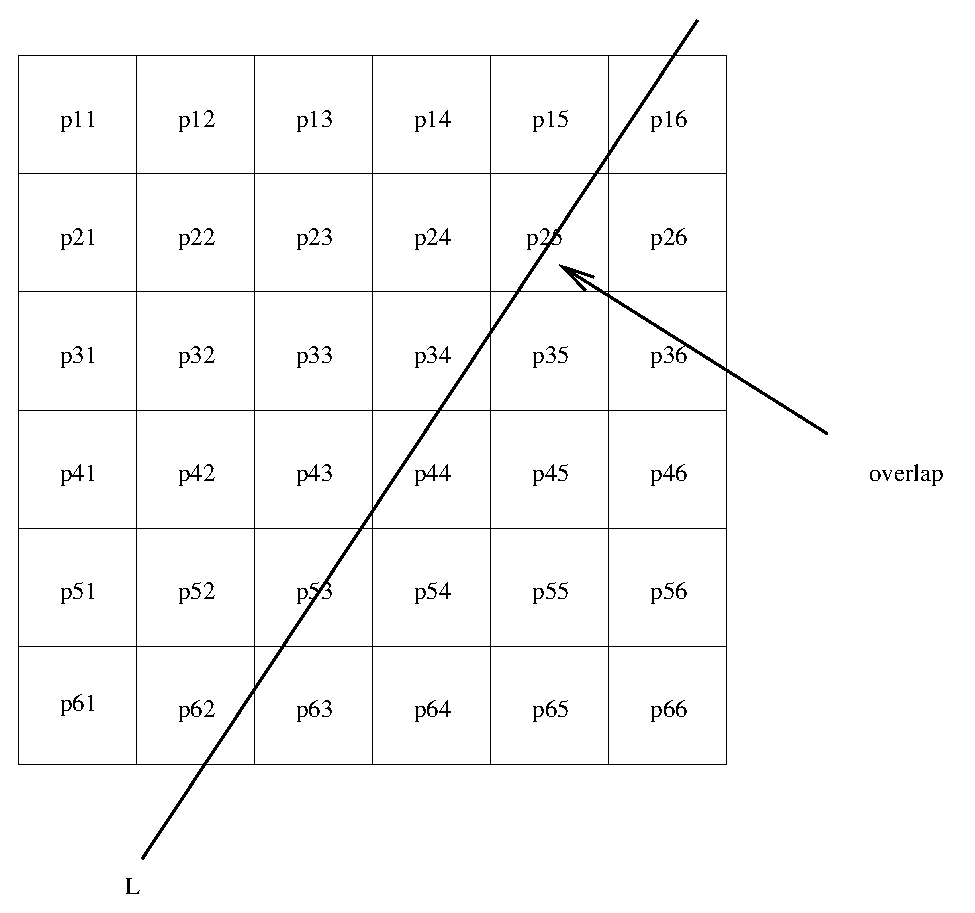
\includegraphics[scale=0.6]{boximage_line.eps}
\caption{Integration over a given line}
\label{boximage}
\end{figure}
For a given set of discrete scan angles and line positions, it is possible to calculate the integral over each line in terms of coefficients for the box-functions. Then one could try to find a set of image/box-function coefficients that gives the least-square error with respect to the measured transform data.  \\
For a box-function image of size $N$x$N$, create a matrix $A$ which entries are given by $A_{i,(m-1)N+n}=a_{m,n}^{L_i}$ where $\{L_i\}$ is a set of lines corresponding to different angles $\theta$ and shifts $u$. If the transform data goes into a vector $B$, indexed over $i$, and the box-function coefficients form the vector $X$ such that $X_{(m-1)N+n}=x_{m,n}$, the following equation should hold
\begin{equation}\label{radoneq}
A\,X=B.
\end{equation}
An equation that is over or under determined depending on the number of scans used. 
For a given line matrix it should be possible to find the least square solution $\widetilde{X}$ to (\ref{radoneq}) with respect to transform data. The image is then recovered in terms of box-functions, which are equivalent to the Haar scaling function, with coefficients that can be fed into the forward wavelet transform. Common de-noising methods such as shrinking could then be utilized. And, if the set of box-functions is replaced with a complete MRA, one could expect to get the recovered image directly into wavelet domain. 
To evaluate this idea, some code was written in Matlab. Unfortunately only garbage solutions were found from the beginning, when the simple backslash operator was used (relying on the characteristic equation, $A^TAx=A^Tb$). It became soon pretty clear that these solutions did not belong to the image domain, due to a large number of negative coefficients, which corresponds to negative pixel values. Instead they were of the form $X=\widetilde{X}+Z$, where $Z\in\mathcal{N}(f)$, i.e. an image solution plus some solution belonging to the null space. These null space solutions consists solely of noise, which could be understood by an example. Imagine a sufficiently large image of box-functions (or pixels) with all coefficients zero, $x_{m,n}=0\ \forall\ m,n$. The transform data of this image is of course zero as well. Then imagine another image of the same size, but with coefficients values corresponding to white noise. The transform values of this noise image will be zero in average, but with random deviation. For lines cutting through many boxes, the value will statistically be of lower absolute value than for lines cutting the corners. Thus, if the noise image is weighted such that the noise close to the corners is of lowest amplitude one gets transform data uniformly close to zero. This is also known as a \emph{ghost image}.    
\begin{figure}[H]
\centering
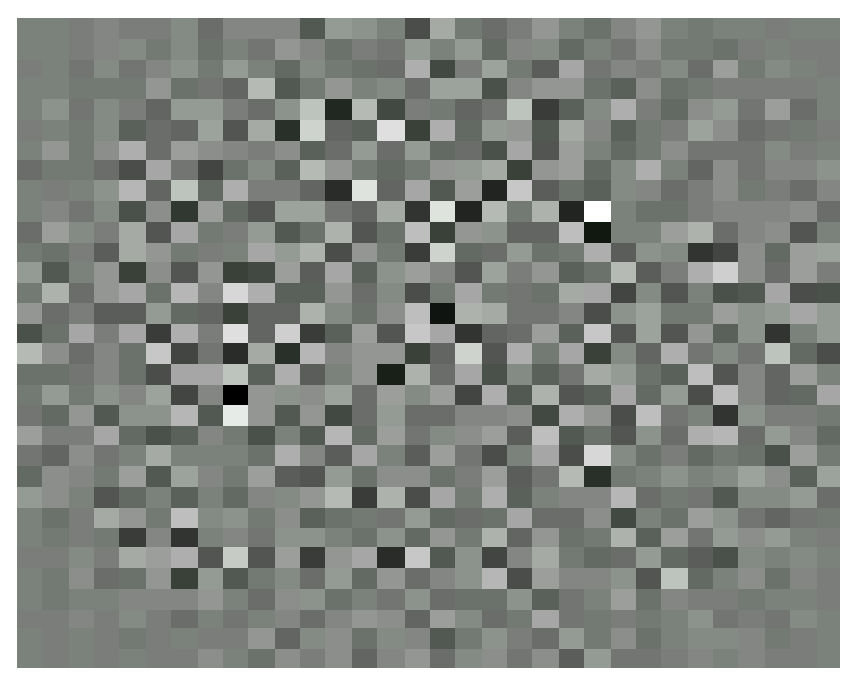
\includegraphics[scale=0.4]{noiseball32.eps}
\caption{A 32 x 32 noisy ghost image}
\label{noiseball}
\end{figure}
Figure \ref{noiseball} shows the noise image that is the typical solution obtained with the simple characteristic equation. The true solution in this case has only a few pixels set in the middle, but these get completely lost in the noise. 
For visualization, the gray scale spans from some negative value and upwards.
One could argue that it should be possible to rotate the transform geometry, i.e. shift the values of $\theta$, to get other least-square images and then add these together to cancel the noise. This might be possible, but one should remember that the matrix $A$ is very large and generating sufficiently many ``rotated copies'' has a very high computational cost. \\
Instead, as a next step, an iterative least-squares optimization algorithm with the constraint of a positive solution was used. Then some reasonably good results were given for small images and a limited number of scans. But unfortunately, due to the fact that the line integral matrix becomes very ill-conditioned, increasing the number of scans/lines over some limit value did not produce a better solution. This can be seen in the figures below.
\begin{figure}[H]
\centering
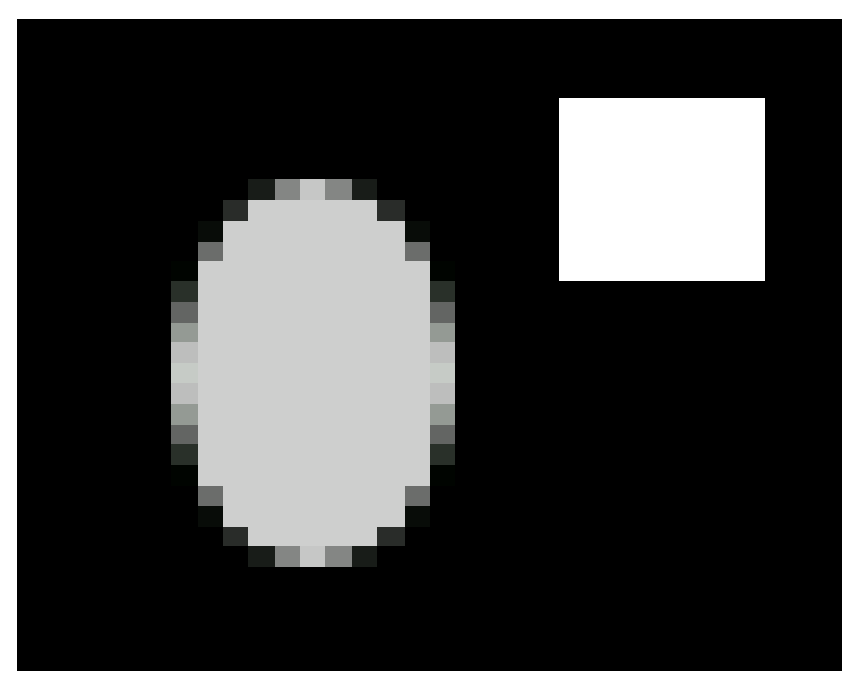
\includegraphics[scale=0.3]{testimage.eps}
\caption{A 32 x 32 test image}
\label{testimage}
\end{figure}
\begin{figure}[H]
\centering
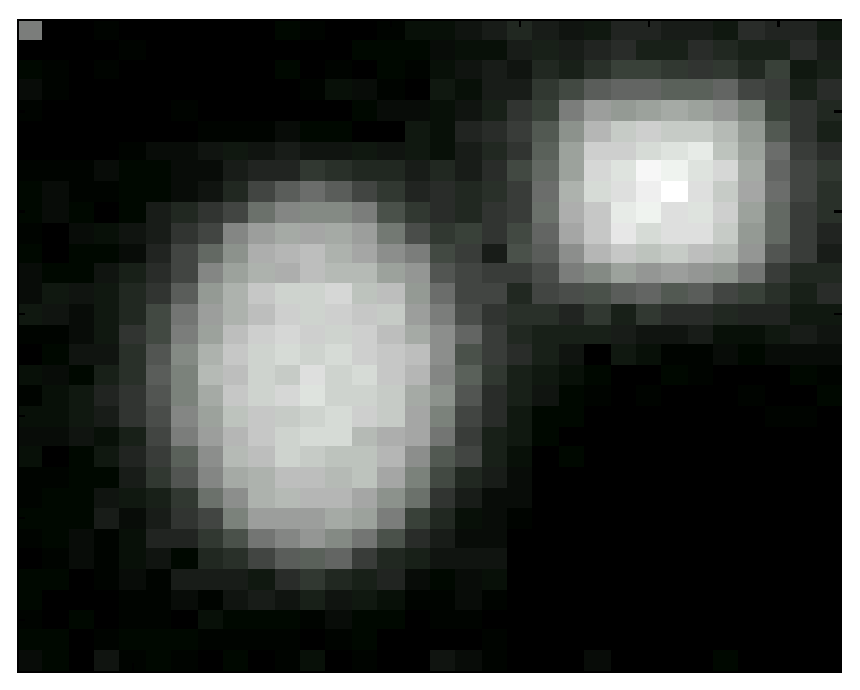
\includegraphics[scale=0.25]{15scans.eps}
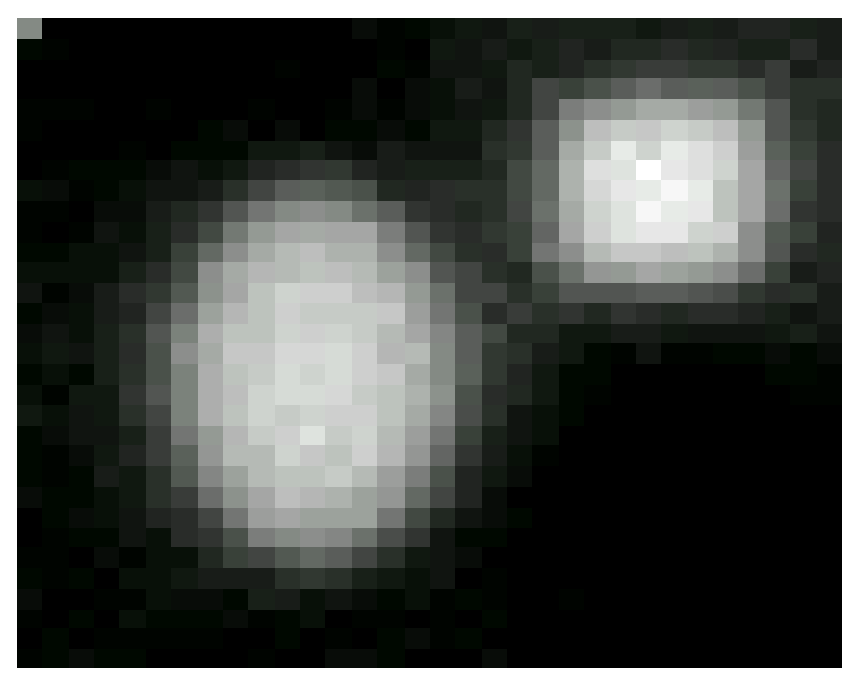
\includegraphics[scale=0.25]{20scans.eps}
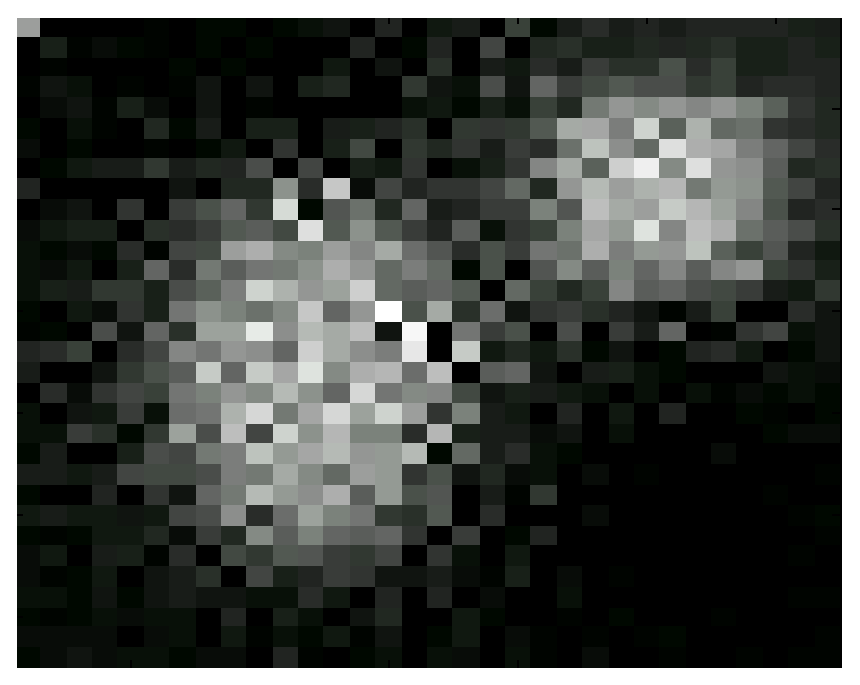
\includegraphics[scale=0.25]{25scans.eps}
\caption{Recovered least-square solutions from 15, 20 and 25 scans respectively}
\label{lsimages}
\end{figure}
In the case with 25 scans, the algorithm stopped when reaching the maximum number of iterations. Increasing this value did not produce a better result. It should also be mentioned that this algorithm with constraints was very costly to perform. Taking it further to wavelet domain would also make little sense, since it would be necessary to include an inverted wavelet transform in each iteration step.\\
A better algorithm to use is \emph{Kaczmarz's method}, \cite{Ladas}\cite{Popa}.
Let $A_m$, for $m=0,\ldots,M$ be operators with null spaces $\mathcal{N}_m$. Let $P_m$ be the operator projecting a vector $x$ onto the set $H_m=\{x\ :\ x=\widetilde{x}+z_m,\ z_m\in\mathcal{N}_m\}$ where $\widetilde{x}$ is a solution satisfying $A_m\widetilde{x}=b_m$ for $m=0,\ldots,M$ and some given $(b_m)$. Then construct the composite operator $P=P_M\ldots P_0$.  Let $x^{(0)}$ be an arbitrary start vector and execute the algorithm
\begin{displaymath}
x^{(J+1)}=Px^{(J)}.
\end{displaymath}
The limit $x^{(\infty)}$ will then be a solution orthogonal to the space $\cap_{m=0}^M\,\mathcal{N}_m$. \\
In the two-dimensional case the algorithm can be visualized by the following figure.
\begin{figure}[H]
\centering
\psfrag{H0}[][]{$H_0$}
\psfrag{H1}[][]{$H_1$}
\psfrag{H2}[][]{$H_2$}
\psfrag{P0}[][]{$P_0$}
\psfrag{P1}[][]{$P_1$}
\psfrag{P2}[][]{$P_2$}
\psfrag{x0}[][]{$x_0$}
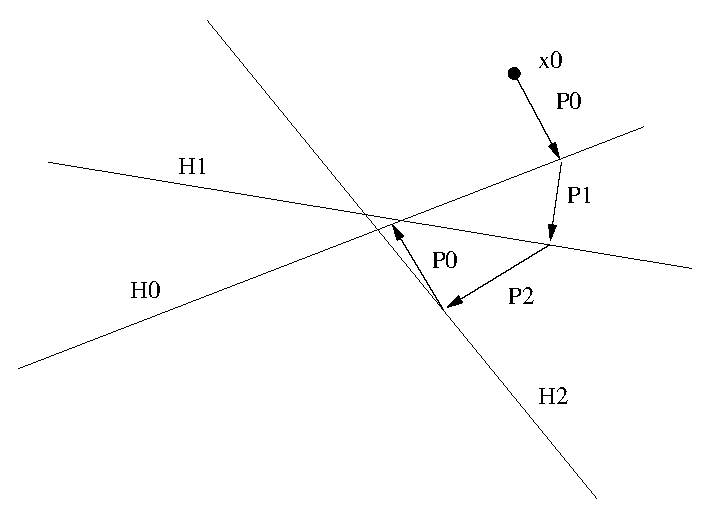
\includegraphics[scale=0.6]{kaczmarz.eps}
\caption{Kaczmarz's method in two dimensions}
\label{boximage}
\end{figure}
Three equations define the spaces $H_0$, $H_1$ and $H_2$. A start vector $x_0$ is projected onto these spaces according to the algorithm. Since there is no point where all three lines cross there is no unique solution, but when the second round of projections is completed it is clear that a solution with small error is given.  \\
In the case with the transform inversion problem, the operators $A_m$ correspond to the rows of the line integral matrix $A$ and the projection operators are given by
\begin{displaymath}
P_m\,X=X-\frac{A_m\,X-B_m}{A_m\,A_m^{\ T}}A_m,
\end{displaymath}
where $B_m$ is the measured transform value corresponding to $A_m$. 
Thus, the result after a few iterations will (hopefully) be a useful least-square solution to the inversion problem (\ref{radoneq}). \\
Below is the result with 15 scans of a 32 x 32 pixels Shepp-Logan phantom image recovered into an MRA of Daubechies wavelets. Only 3 iterations were used of Kaczmarz's algorithm. Hard thresholding has been applied to the coefficients before inversion into image domain.
\begin{figure}[H]
\centering
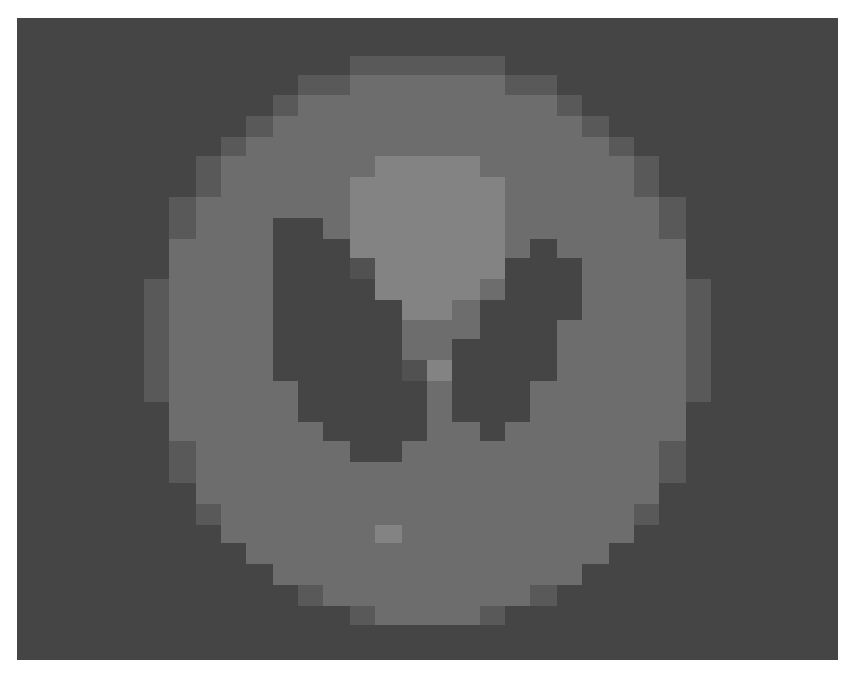
\includegraphics[scale=0.3]{phantom32orig.eps}
\caption{32 x 32 Shepp-Logan phantom image}
\label{SL32origimage}
\end{figure}

\begin{figure}[H]
\centering
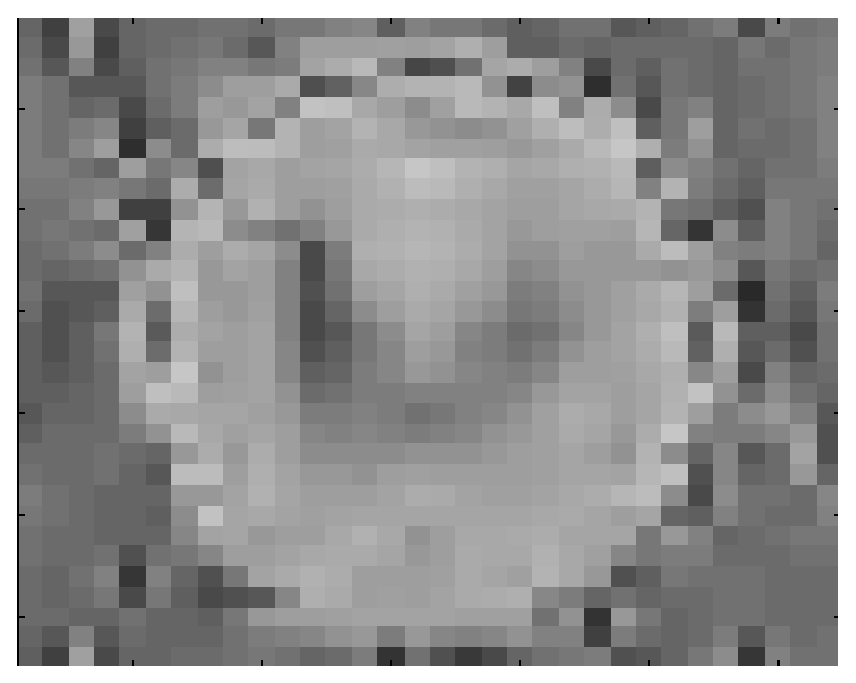
\includegraphics[scale=0.3]{phantom32_15_3_thresh_daubechies6.eps}
\caption{Recovered image}
\label{SL32recovered}
\end{figure}

When the same type of phantom image in 64 x 64 pixels was subject to 40 scans, the following image was recovered, before and after some hard thresholding of the wavelet coefficients.
\begin{figure}[H]
\centering
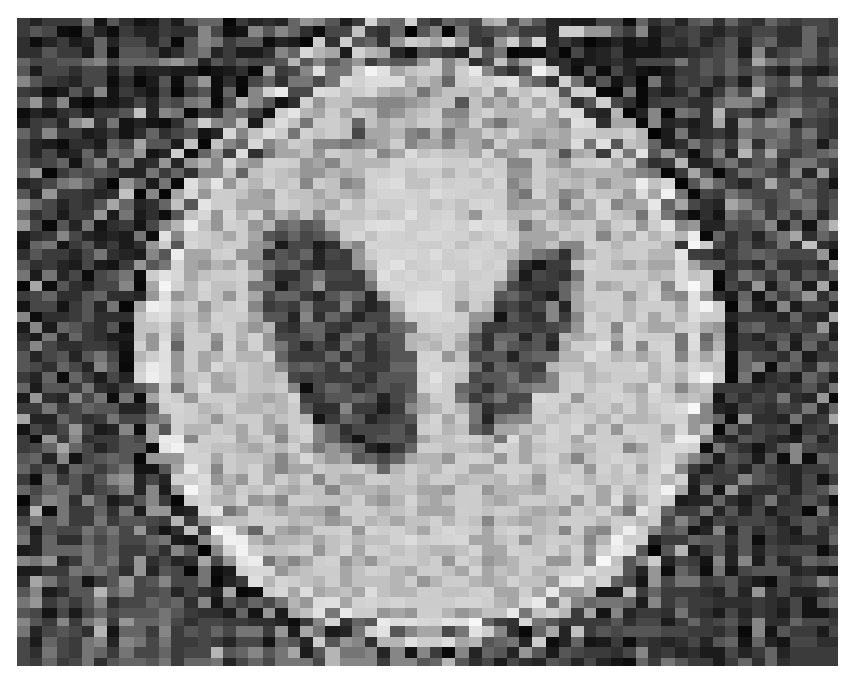
\includegraphics[scale=0.5]{phantom64_40_4.eps}
\caption{Recovered image}
\label{SL64recovered}
\end{figure}
\begin{figure}[H]
\centering
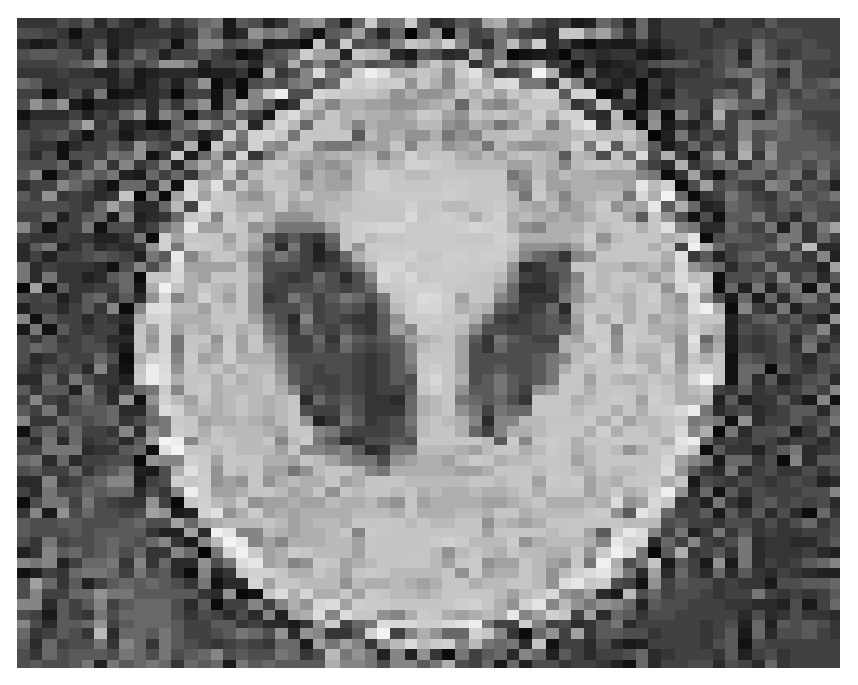
\includegraphics[scale=0.5]{phantom64_40_4_thresh.eps}
\caption{Recovered image after thresholding}
\label{SL64recovered}
\end{figure}
Apart from denoising aspects, recovering the image directly into wavelet domain might not seem to provide any obvious benefits, but it opens up for local and/or adaptive reconstruction. For instance, only wavelet scales of interest could be used for computation of the line integral matrix.\\
Common to the methods of least-square recovery is of course that they rely on the ability to generate a geometry for the line integral matrix that closely resembles the practical measurements. The associated difficulties has not been studied in connection to this work.

\begin{flushright}
$\Box$ 
\end{flushright}





\begin{thebibliography}{99}
\bibitem{Anderson}D. V. Anderson, \emph{Speech Analysis and Coding using a Multi-Resolution Sinusoidal Transform}, IEEE 1996 Int. Conf. on Acoustics, Speech, and Signal Processing
\bibitem{Bergh}J. Bergh, F. Ekstedt, M. Lindberg, \emph{Wavelets}, Studentlitteratur 1999
\bibitem{Beylkin1}G. Beylkin, R. Coifman, V. Rokhlin, \emph{Fast Wavelet Transforms and Numerical Algorithms I.}
\bibitem{Beylkin2}G. Beylkin, \emph{On the representation of operators in bases of compactly supported wavelets}, SIAM Journal on Numerical Analysis vol 29, 1992, pp. 1716-1740  
\bibitem{Christov}I. Christov, \emph{Wavelet-Galerkin Methods for Partial Differential Equations}, Matrix Analysis and Wavelets REU, TAMU, 2003
\bibitem{Dahmen}W. Dahmen, C. A. Micchelli, \emph{Using the refinement equation for evaluating integrals of wavelets}, SIAM Journal on Numerical Analysis vol 30, 1993, pp. 507-537 
\bibitem{Debnath}L. Debnath, P. Mikusinski, \emph{Introduction to Hilbert Spaces with Applications}, Academic Press 1999
\bibitem{Donoho}D. L. Donoho, \emph{Nonlinear Solution of Linear Inverse Problems by Wavelet-Vaguelette Decomposition}, Applied and Computational Harmonic Analysis vol 2, 1995, pp. 101-126 
\bibitem{Eriksson}K. Eriksson, D. Estep, P. Hansbo, C. Johnson, \emph{Computational Differential Equations}, Studentlitteratur 1996
\bibitem{Goswami}J. C. Goswami, A. K. Chan, \emph{Fundamentals of Wavelets. Theory, Algorithms, and Applications}, Wiley Interscience 1999
\bibitem{Jawerth}B. Jawerth, W. Sweldens, \emph{Wavelet Multiresolution Analyses adapted for the Fast Solution of Boundary Value Ordinary Differential Equations}, available online:\\ \verb| http://cm.bell-labs.com/who/wim/|
\bibitem{Johnson}B. R. Johnson et al., \emph{Quadrature integration for orthogonal wavelet systems}
\bibitem{Kunoth}A. Kunoth, \emph{Computing Refinable Integrals - Documentation of the Program}, 1995, available online:\\ \verb|http://www.iam.uni-bonn.de/~kunoth/papers/papers.html|
\bibitem{Ladas}K. T. Ladas, A. J. Devaney, \emph{Generalized ART algorithm for diffraction tomography}, Inverse Problems vol 7, no. 1, pp. 109-125, February 1991
\bibitem{Lee&Lucier}N-Y Lee, B. J. Lucier, \emph{Wavelet Methods for Inverting the Radon Transform with Noisy Data}, IEEE Trans. on Image Processing vol 10, No 1, January 2001
\bibitem{Li}X. Li, B. Hu, X. Ling, X. Zeng, \emph{A wavelet balance approach for steady-state analysis of nonlinear circuits}, IEEE Trans. on Circuits and Systems - I (TCAS-I), vol. 49, no. 5, pp. 689-694, May 2002
\bibitem{Lynn}P. A. Lynn, W. Fuerst, \emph{Introductory Digital Signal Processing with Computer Applications}, second edition, John Wiley \& Sons 1998 (reprint of 1994)
\bibitem{Popa}C. Popa, R. Zdunek, \emph{Kaczmarz extended algorithm for tomographic image reconstruction from limited-data}, Mathematics and Computers in Simulation, vol. 65, Issue 6, pp. 557-655, May 2004
\bibitem{Soveiko}N. Soveiko, M. Nakhla, \emph{Steady State Analysis of Multitone Nonlinear Circuits in Wavelet Domain}, IEEE Trans. Microwave Theory Tech., April 2004
\bibitem{Strang}G. Strang, T. Nguyen, \emph{Wavelets and Filter Banks}, Wellesley - Cambridge Press 1996


\end{thebibliography}

\end{document}


